\chapter{Diodi}

\renewcommand\thesection{\Roman{section}}

\section{Caratteristica I-V di un diodo}

\textbf{Obiettivo:} ricavare le caratteristiche I-V di un diodo al silicio e di un diodo LED.

\paragraph{Strumentazione:}
\begin{enumerate}
    \item un generatore di tensione;
    \item un diodo al silicio e un diodo LED;
    \item una resistenza tra $\SI{0.5}{\kilo\Omega}$ e $\SI{5}{\kilo\Omega}$;
    \item un amperometro e un voltmetro.
\end{enumerate}

\paragraph{Procedura:}
\begin{enumerate}
    \item costruire il circuito;
    \begin{figure}[h]
        \centering
        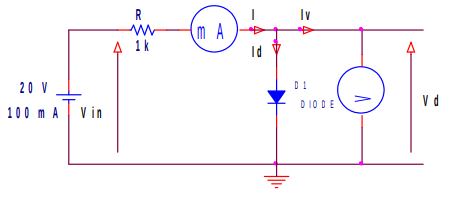
\includegraphics[width=0.6\linewidth]{Immagini/EXP5 - IV diodo.png}
        \caption{circuito da costruire}
        \label{fig: EXP5 - IV diodo}
    \end{figure}
    \item per il diodo al silicio, variare la tensione in ingresso e costruire il grafico di $I(V_d)$, dove $V_d$ è la tensione del diodo;
    \item effettuare una regressione dei dati con l'equazione di Shockley
    \begin{equation}
    I_{d} = I_{s} \left( e^{V_{d}/\eta V_{T}} - 1 \right),\quad V_T=\frac{kT}{e}=\SI{26}{mV}.
    \end{equation}
    \item Dai dati sperimentali si può ricavare $\eta$ che per diodi al silicio vale circa 2, per poi diminuire ad alte correnti di conduzione del diodo.
    \item il diodo LED ha invece una componente resistiva non trascurabile, che fa sì che l'equazione di Shockley non descriva bene l'andamento della corrente ad alti valori. Ai capi del diodo è presente una caduta di potenziale $V_{d} = R_dI_d$. Non è possibile ricavare l'espressione analitica di $I_d(V_d)$, ma è possibile ricavare $V_d(I_d)$, invertendo la relazione di Shockley ed aggiungendo il termine resistivo
    \begin{equation}
        V_d=\eta V_T\ln{\left(\frac{I_d}{I_s}+1\right)}+R_dI_d.
    \end{equation}
\end{enumerate}

\section{Raddrizzamento di una semionda}

\paragraph{Obiettivo:} rendere la tensione ``pulsata'' costante nel tempo tramite l'aggiunta di un filtro RC.

\paragraph{Strumentazione:}
\begin{enumerate}
    \item un generatore di funzioni;
    \item un diodo al silicio;
    \item un condensatore di $\SI{10}{\micro\farad}$ e una resistenza di $\SI{1}{\kilo\ohm}$ per creare un filtro RC;
    \item un oscilloscopio.
\end{enumerate}

\paragraph{Procedura:}
\begin{enumerate}
    \item applicando all'ingresso di un circuito, con in serie il diodo e una resistenza, una tensione sinusoidale, si può osservare con l'oscilloscopio che la tensione di uscita contiene solo la semionda positiva;
    \begin{figure}[h]
        \centering
        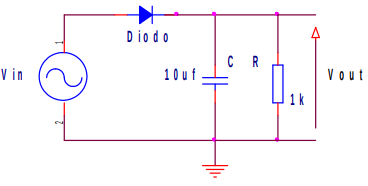
\includegraphics[width=0.6\linewidth]{Immagini/EXP5 - semionda.png}
        \caption{circuito per il raddrizzamento della semionda.}
        \label{fig: EXP5 - semionda}
    \end{figure}
    \item per renderla costante nel tempo si deve aggiungere un condensatore in parallelo alla resistenza, in modo da formare un filtro RC;
    \item verificare l'andamento della tensione in uscita.
\end{enumerate}

\setcounter{section}{0}
\renewcommand\thesection{\Alph{section}}

\section{Modellizzazione di un diodo}
Dalla caratteristica del diodo al silicio si osserva che esso comincia a condurre per tensioni $V_d$ maggiori di 0.5 V ed essendo un andamento esponenziale la corrente sale molto velocemente con la tensione applicata. Con questa osservazione per semplificare i calcoli del circuito, si può sostituirlo con dei modelli in modo da poter applicare la legge di Ohm. Per un diodo ideale:
\begin{itemize}
    \item se conduce, sostituirlo con un cortocircuito;
    \item  se non conduce, sostituirlo con un circuito aperto.
\end{itemize}
\begin{figure}[h]
    \centering
    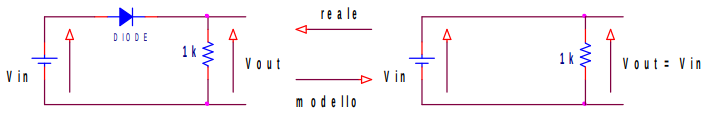
\includegraphics[width=0.9\linewidth]{Immagini/EXP5 - diodo (conduzione).png}
    \caption{diodo in conduzione.}
    \label{fig: EXP5 - diodo (conduzione)}
\end{figure}
\begin{figure}[h]
    \centering
    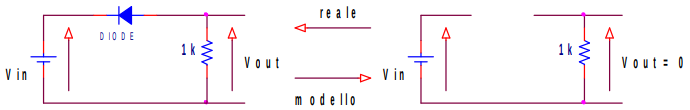
\includegraphics[width=0.9\linewidth]{Immagini/EXP5 - diodo (no conduzione).png}
    \caption{diodo non in conduzione.}
    \label{fig: EXP5 - diodo (no conduzione)}
\end{figure}
Un altro modello molto usato è quello di sostituire il diodo in conduzione con una
resistenza $r_f\approx\SI{10}{\ohm}$ ed un generatore $V_{\gamma}\approx\SI{0.5}{V}$ collegati fra loro in serie
\begin{figure}[h]
    \centering
    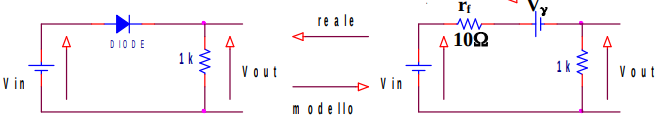
\includegraphics[width=0.9\linewidth]{Immagini/EXP5 - modello diodo (conduzione).png}
    \caption{modello per un diodo in conduzione.}
    \label{fig: EXP5 - modello diodo (conduzione)}
\end{figure}

La tensione in uscita diventa $V_{out}=V_{in}-V_{\gamma}-Ir_f$, ma in molti casi si considera $r_f=0$ e sostituire $V_\gamma$ con $V_{\sigma}=\SI{0.7}{V}$ ottenendo $V_{out}=V_{in}-0.7$. Se il diodo è polarizzato inversamente esso può essere sostituito semplicemente da una resistenza $r_f$ di valore molto elevato dell'ordine di decine di M$\Omega$.